  \begin{itemize}
  \item \textit{MIRGE-Com} Overview
%    \begin{itemize}
%    \item Pieces/anatomy
%    \item Symbolic infrastructure
%    \item Verification of NS w/MMS  (and others)
%    \end{itemize}
  \item Testing \& Verification
  % \item Development process
%    \begin{itemize}
%    \item Development process (production)
%    \item Prediction-targeted testing
%       \item $\nabla{Y}$ boundary condition issue post-mortem
%    \end{itemize}
  \item Performance snapshot
%    \begin{itemize}
%    \item Current and historical
%    \item Needed for prediction
%    \end{itemize}
  \item Next for \mirgecom
  % \item Wrap-up \& next steps
%    \begin{itemize}
%    \item Transport
%    \item ESDG
%    \item Testing, testing, and testing
%    \item Challenges and Risks (testing holes, performance challenge, debugging challenge)
%    \end{itemize}
\end{itemize}

  \begin{frame}\frametitle{Symbolic Infrastructure for Fluids}
  \begin{center}
  %Evolution equation:
  Compressible Navier--Stokes for reactive mixtures:
  \begin{equation*}
    \frac{\partial\mathbf{Q}}{\partial{t}} + \nabla \cdot (\mathbf{F}^I - \mathbf{F}^V) - \mathbf{S} = 0
  \end{equation*}
  % With chemistry source terms:
  % \begin{equation*}
  %  \mathbf{S} = [ 0, 0, 0, 0, 0, W_k\dot{\omega_k} ]
  %\end{equation*}
    Where state vector $\mathbf{Q}$, fluxes $\mathbf{F}^I$, $\mathbf{F}^V$ , and sources $\mathbf{S}$ are given by:
 \begin{equation*}
      \begin{bmatrix}
        \rho\\\rho{E}\\\rho\vec{v}\\\rho{Y}_\alpha\end{bmatrix},\quad
      \begin{bmatrix} \rho\vec{v}\\(\rho{E} +
        p)\vec{v}\\\rho(\vec{v} \otimes \vec{v}) +
        p\delta_{ij}\\\rho{Y}_\alpha\vec{v}\end{bmatrix}, \quad
       \begin{bmatrix} 0\\(\mathbf{\tau} \cdot \vec{v} - \mathbf{q})\\\mathbf{\tau}\\-\mathbf{J}_\alpha\end{bmatrix},\quad
       \begin{bmatrix} 0\\0\\0\\W_\alpha\dot{\omega}_\alpha\end{bmatrix}
 \end{equation*}
 $\tau = \mu\left(\nabla\vec{v} + (\nabla\vec{v})^T\right) + \left(\mu_b - \frac{2\mu}{3}\right)\left(\nabla \cdot \vec{v}\right)$\\
\vspace{5pt}
$\mathbf{J}_\alpha = -\rho D_{(\alpha)} \nabla(Y_\alpha)$ \quad and \quad $\mathbf{q} = -\kappa\nabla{T} + h_\alpha\mathbf{J}_\alpha$\\
\vspace{10pt}
    The mixture gas model (EOS) provides $\rightarrow~~(p,T,e,\mu,\kappa,D_{\alpha}, \omega_\alpha, h_\alpha)(\mathbf{Q})$
  \end{center}
  \begin{tikzpicture}[remember picture, overlay]
    \fill <2> [fill=white, opacity=0.8] (current page.south west) + (0.5,0.5) rectangle (12.5,7.5);
    \node <2> [inner sep=0pt] at (current page.center) {
      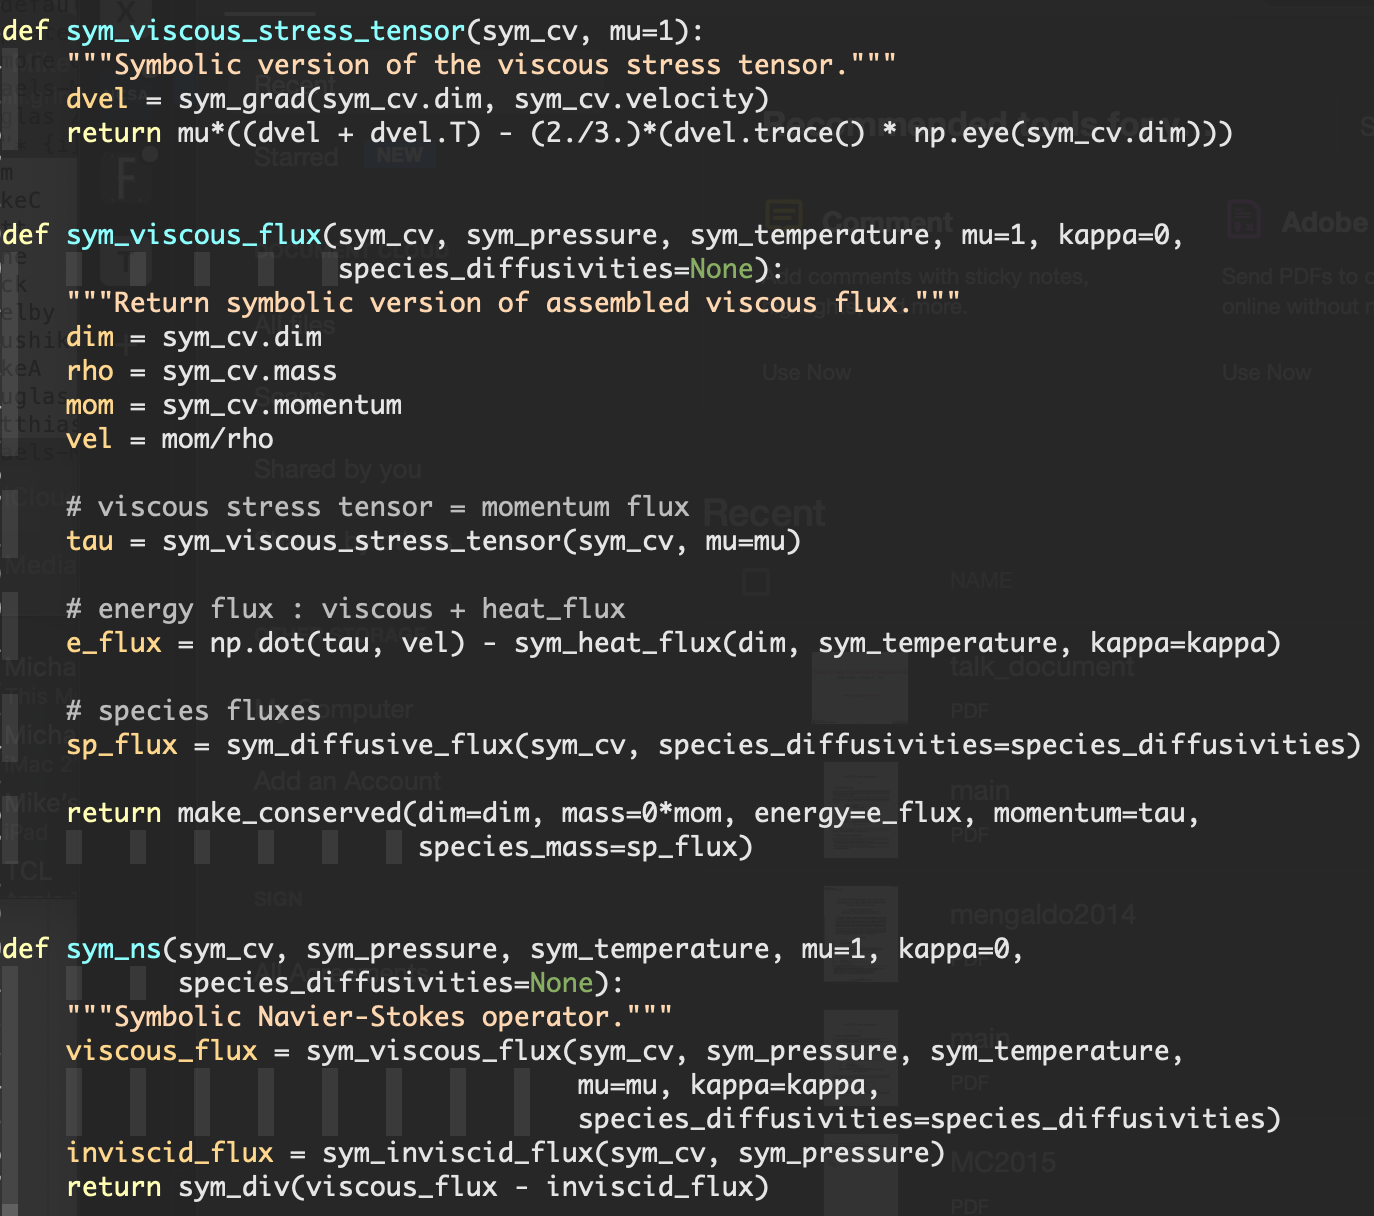
\includegraphics[width=.5\textwidth]{Figures/mtc/SymbolicInfrastructureCode.png}
    };
  \end{tikzpicture}
\end{frame}

\begin{frame}\frametitle{Symbolic Infrastructure for Fluid Component Testing}
\center{What's it good for?}
\begin{itemize}
\item Fluid component verification testing
\item Specify analytic test functions and 
\item Evaluate convergence of MIRGE components to exact/analytic solution
\end{itemize}
\begin{center}
  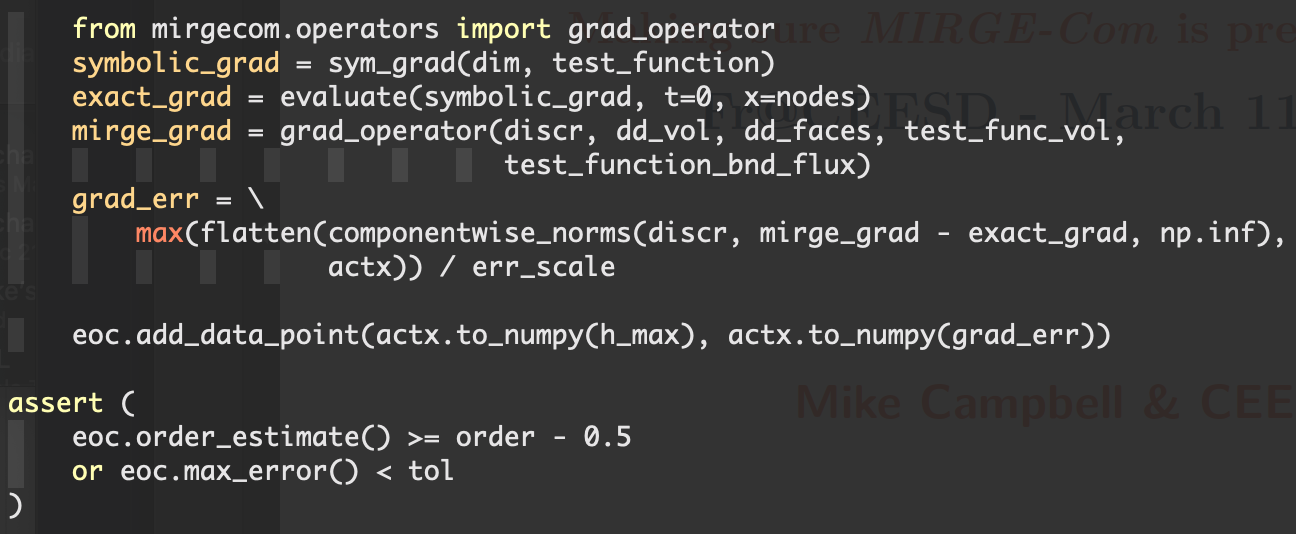
\includegraphics[width=.6\textwidth]{Figures/mtc/ComponentVerifCode.png}
\end{center}
\begin{itemize}
\vspace{-10pt}
\item and ... method of manufactured solutions (MMS)
\end{itemize}
\end{frame}

\begin{frame}\frametitle{Method of Manufactured Solutions in \mirgecom{}}
\begin{itemize}
\item Craft an analytic solution, $\mathnormal{CV}_S: = \left[\rho=\phi_m, \rho{E}=\phi_e, \rho\mathbf{V}=\mathbf{\phi}_p\right]$:
\end{itemize}
\begin{center}
  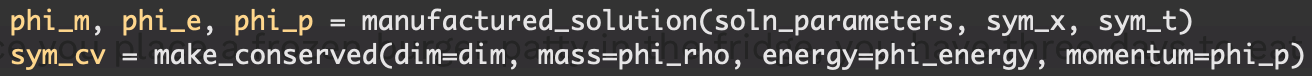
\includegraphics[width=.6\textwidth]{Figures/mtc/CreateSymbolicSolution.png}
\end{center}
\begin{itemize}
\item Compute source terms, $S_S = (\frac{d}{\mathnormal{dt}})_S(\mathnormal{CV}_S) - \mathnormal{NS}_S(\mathnormal{CV}_S)$:
\end{itemize}
\begin{center}
  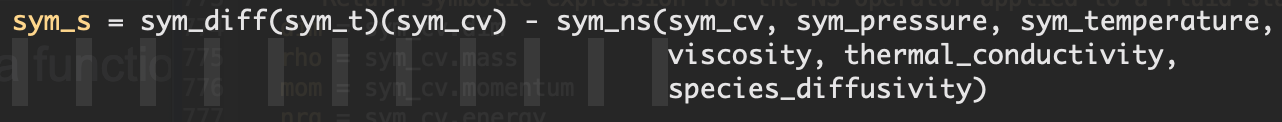
\includegraphics[width=.6\textwidth]{Figures/mtc/CalculateSymbolicSources.png}
\end{center}
\begin{itemize}
\item Evaluate the source term, $S_\text{num} = \text{Eval}(S_S)$, and modify the NS RHS: 
\end{itemize}
\begin{center}
  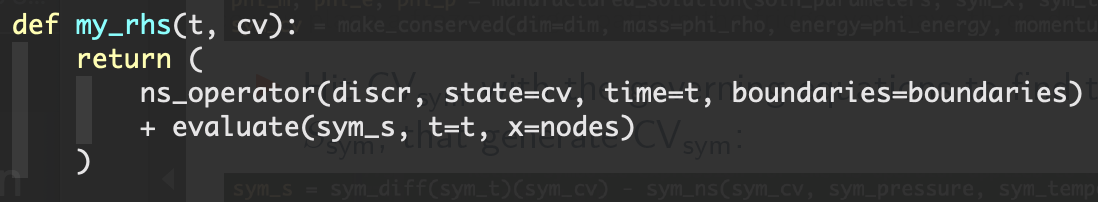
\includegraphics[width=.6\textwidth]{Figures/mtc/NumRHS.png}
\end{center}
\begin{itemize}
\item Evaluate mesh convergence and accuracy as usual
%      \begin{itemize}
%      \item Solution initialized to numerical $\text{CV}_\text{sym}$, and
%      \item Exact/analytic prescribed boundary conditions
%      \end{itemize}
\end{itemize}
\begin{center}
  \begin{minipage}{.8\textwidth}
  \paper{\sPI{P.~Roache}, ``Code Verification by the Method of Manufactured Solutions,'' \textit{J. Fluids Eng.} \textbf{124} 4 (2002)}
  \end{minipage}
 \end{center}
% https://doi.org/10.1115/1.1436090
% Patrick J. Roache Code Verification by the Method of Manufactured Solutions
%\item Advantages:
%      \begin{itemize}
%      \item Simplicity (easily understood and implemented)
%      \item Exercises selected, or all terms
%      \item Tests the whole code - all components in an integrated fashion - component-only tests leave many questions and holes
%      \item Highly sensitive for detecting mistakes
%      \end{itemize}
%\end{itemize}
\end{frame}

\begin{frame}\frametitle{CNS Verification with MMS}
  \begin{multicols}{2}
  \begin{itemize}
  \item Integrated MMS: Roy Solution
  \item 2,3 dimensions, sub/super-sonic
  \item Exact boundaries
  \item Exercises all CNS equations (single gas)
  \end{itemize}
  \begin{center}
  \vspace*{-5pt}
  \tiny{Roy MMS components}
  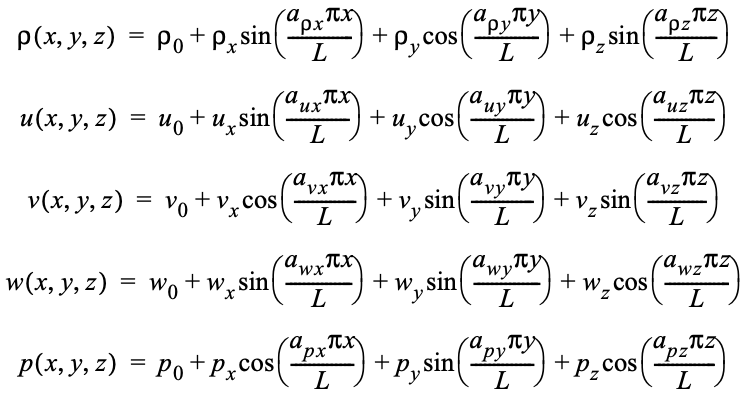
\includegraphics[width=.4\textwidth]{Figures/mtc/RoySoln.png}
  \end{center}
  \columnbreak
  \vspace*{-35pt}
  \begin{center}
  \tiny{Pressure contours for 3D subsonic Roy MMS.}
  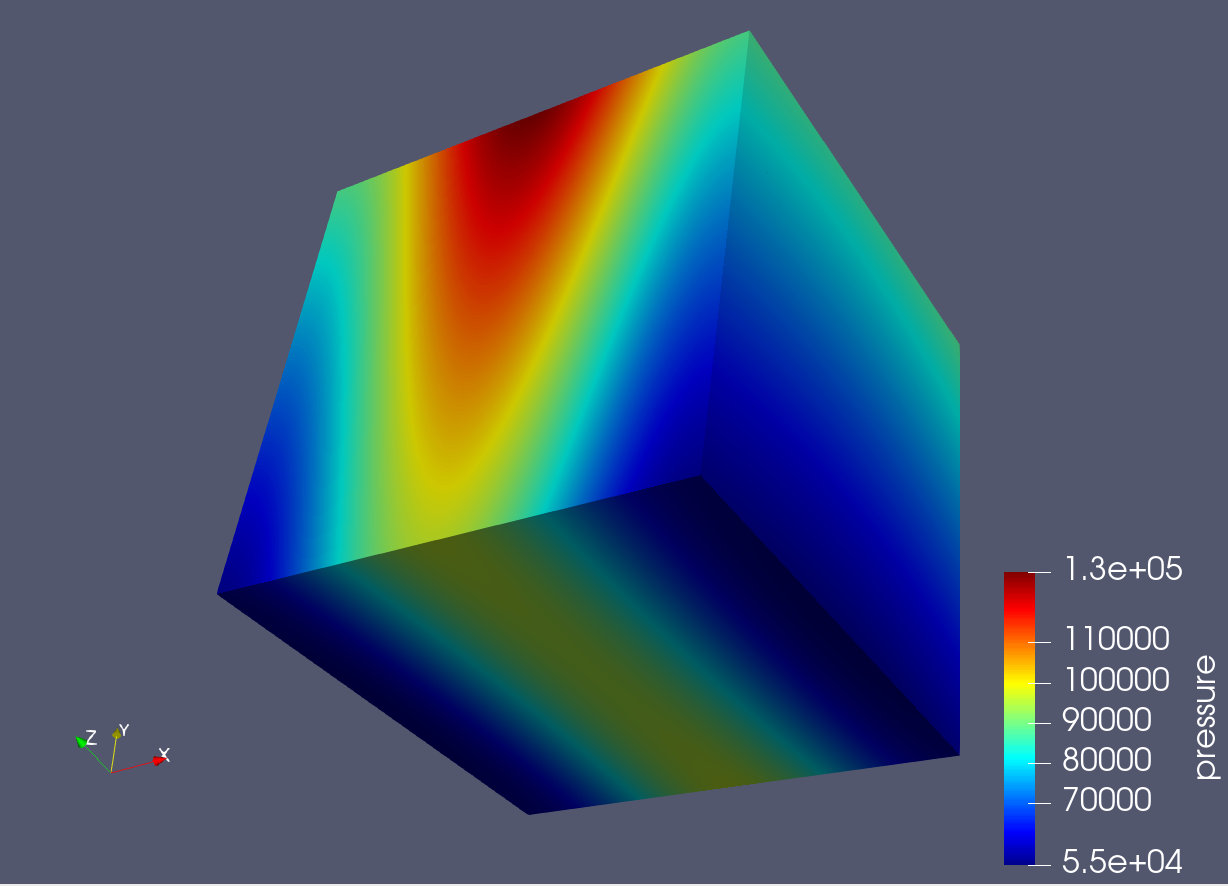
\includegraphics[width=.3\textwidth]{Figures/mtc/RoyPressure3D.png}\\
  \vspace*{10pt}
  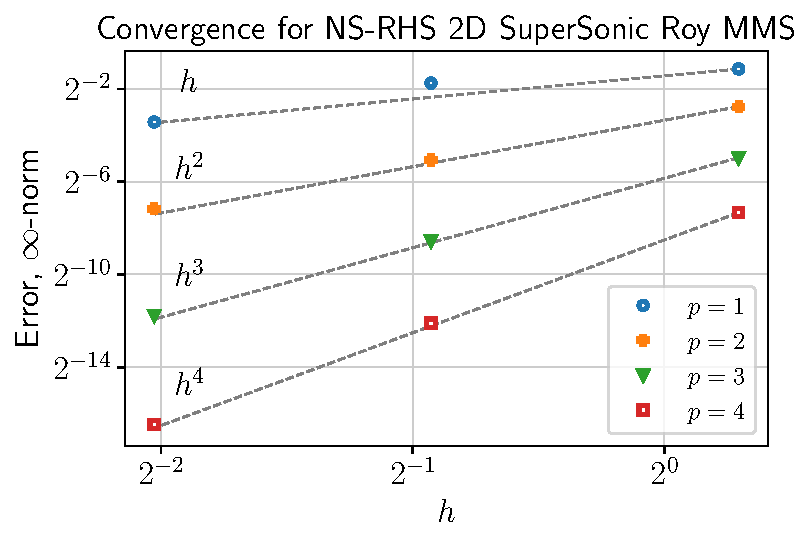
\includegraphics[width=.35\textwidth]{Figures/mtc/roy_convergence.pdf}
  \end{center}
  \end{multicols}
  \begin{center}
  \vspace*{-10pt}
  \begin{minipage}{.8\textwidth}
  \paper{\sPI{C.~Roy, T.~Smith, and C.~Ober}, ``Verification of a Compressible CFD Code using the Method of Manufactured Solutions,'' \textit{AIAA} Paper 2002-3110 (2002)}
  \end{minipage}
%    \prj\tiny{Roy, Verification of a Compressible CFD Code using the Method of Manufactured Solutions, AIAA Paper 2002-3110 \href{https://doi.org/10.2514/6.2002-3110}}
  \end{center}
\end{frame}

\begin{frame}\frametitle{Testing and Verification}
\begin{multicols}{2}
  \begin{itemize}
  \item Built-in, automated tests:
    \begin{itemize}
    \item Unit example: Planar Poiseuille
    \begin{itemize}
    \item CNS Single gas or mixture EOS
    \item Adiabatic noslip, inflow, outflow boundaries
    \end{itemize}
    \item Integrated example: Species advection-diffusion
    \begin{itemize}
    \item Inert species components of CNS
    \item Periodic or exact boundaries
    \end{itemize}
    \item Prediction-relevant testing \prj{\tiny}{M. Anderson}
    \end{itemize}
\item New validation tests; e.g., flames and stand-burners \prj{\tiny}{T. Ricciardi}
\item Longer running cases become examples
%\item Address needs:
%      \begin{itemize}
%      \item Documentation, organization, standardization? of our current testing
%      \item More tests (of course):
%            \begin{itemize}
%            \item Prediction-relevant capability tests
%            \item Prediction-relevant issue reproducers,
%            \item and manufactured solution tests
%            \end{itemize}
%      \end{itemize}
\end{itemize}
\columnbreak
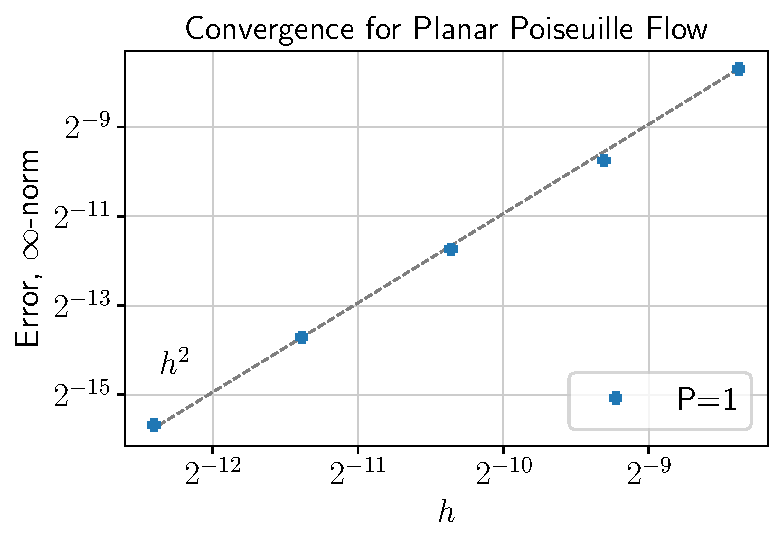
\includegraphics[width=.35\textwidth]{Figures/mtc/poiseuille-convergence.pdf}
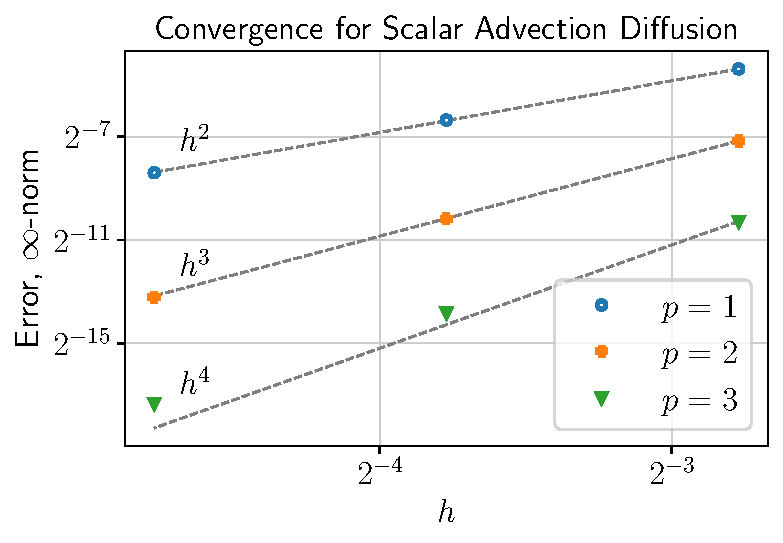
\includegraphics[width=.35\textwidth]{Figures/mtc/advdiff_convergence_bigger.pdf}
\end{multicols}
  \begin{tikzpicture}[remember picture, overlay]
    \fill <2> [fill=white, opacity=0.8] (current page.south west) + (0.5,0.5) rectangle (12.5,7.5);
    \node <2> [inner sep=0pt] at (current page.center) {
      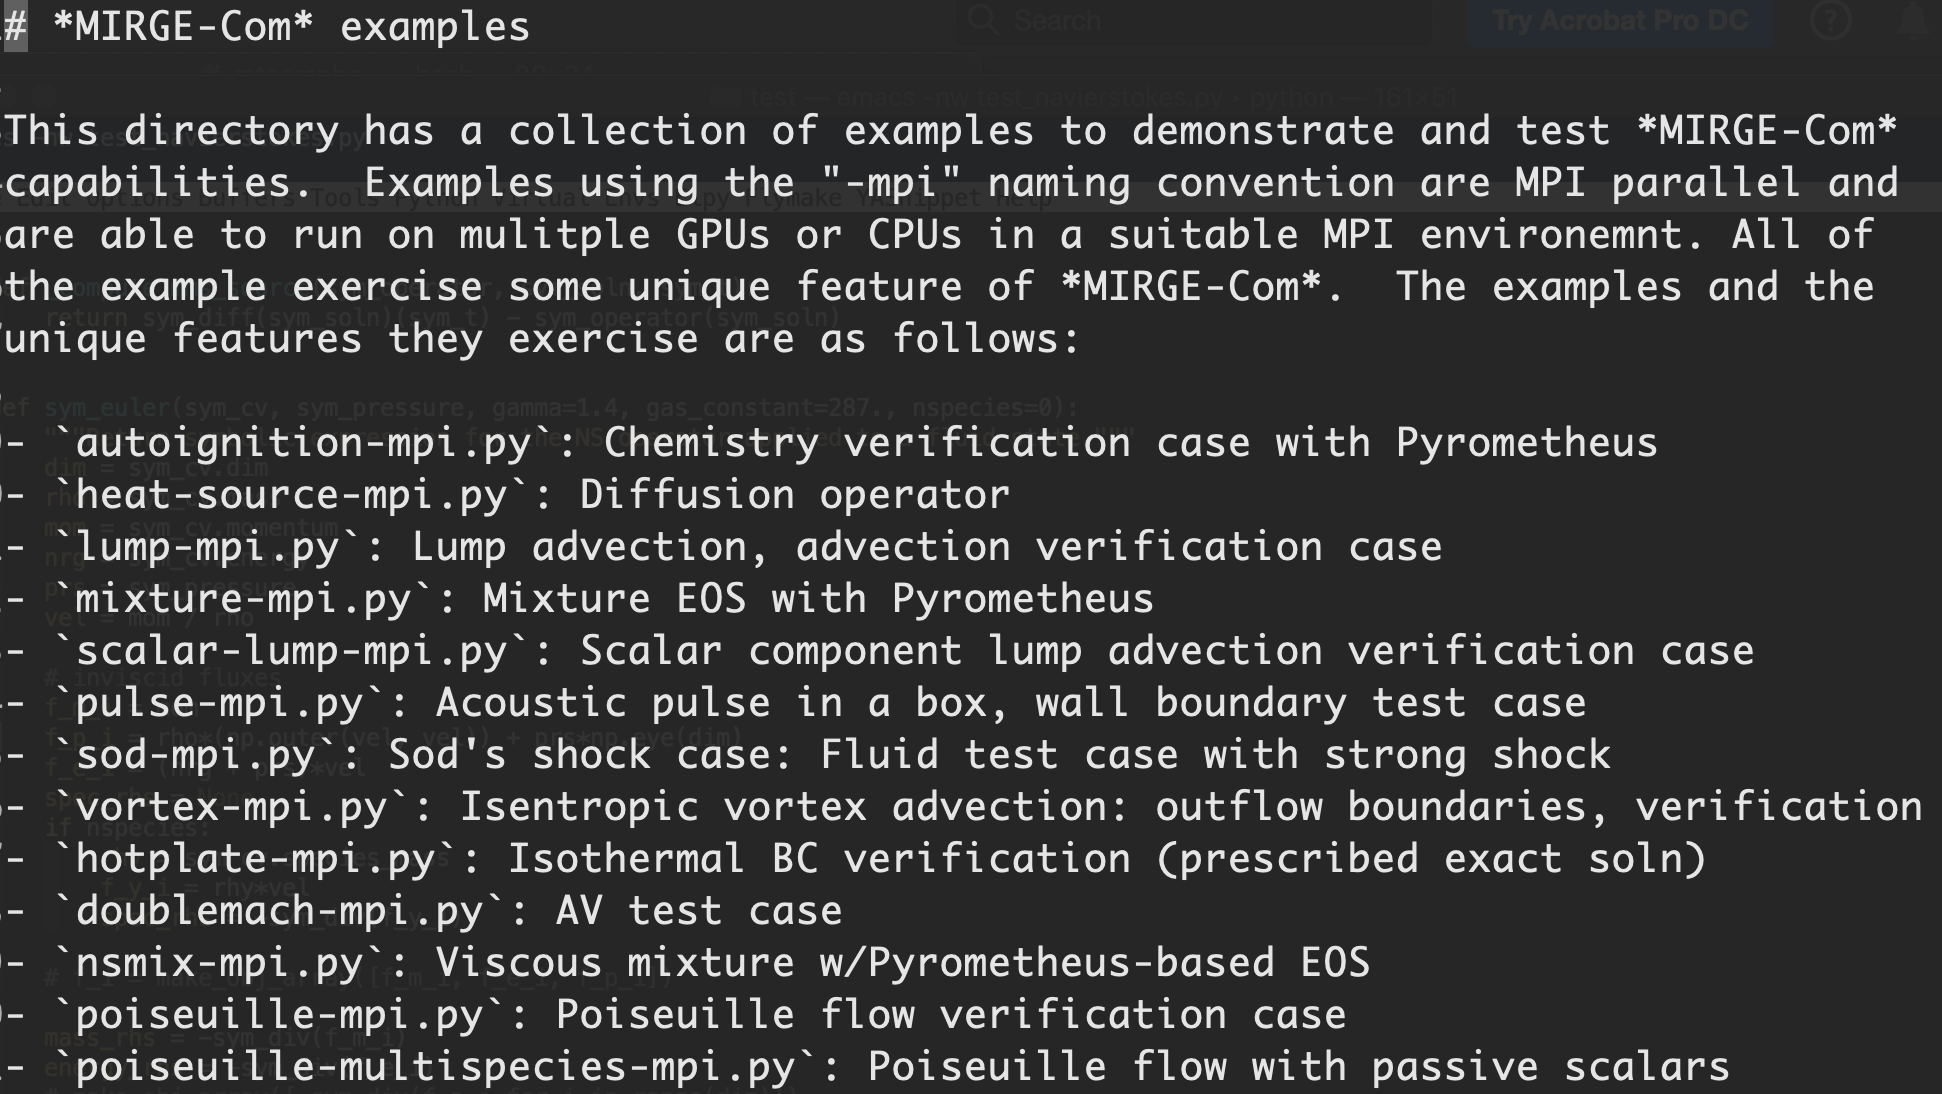
\includegraphics[width=.7\textwidth]{Figures/mtc/ExamplesReadme.png}
    };
  \end{tikzpicture}
\end{frame}

%\begin{frame}\frametitle{V\&V Testing}
%\begin{multicols}{2}
%\begin{itemize}
%\item Unit example: Poiseuille
%\item Integrated example: Species advection-diffusion
%\item New tests; e.g. flames and stand-burners \prj{\tiny}{T. Ricciardi}
%\item Prediction-relevant testing \prj{\tiny}{M. Anderson}
%%\item Address needs:
%%      \begin{itemize}
%%      \item Documentation, organization, standardization? of our current testing
%%      \item More tests (of course):
%%            \begin{itemize}
%%            \item Prediction-relevant capability tests
%%            \item Prediction-relevant issue reproducers,
%%            \item and manufactured solution tests
%%            \end{itemize}
%%      \end{itemize}
%\end{itemize}
%\columnbreak
%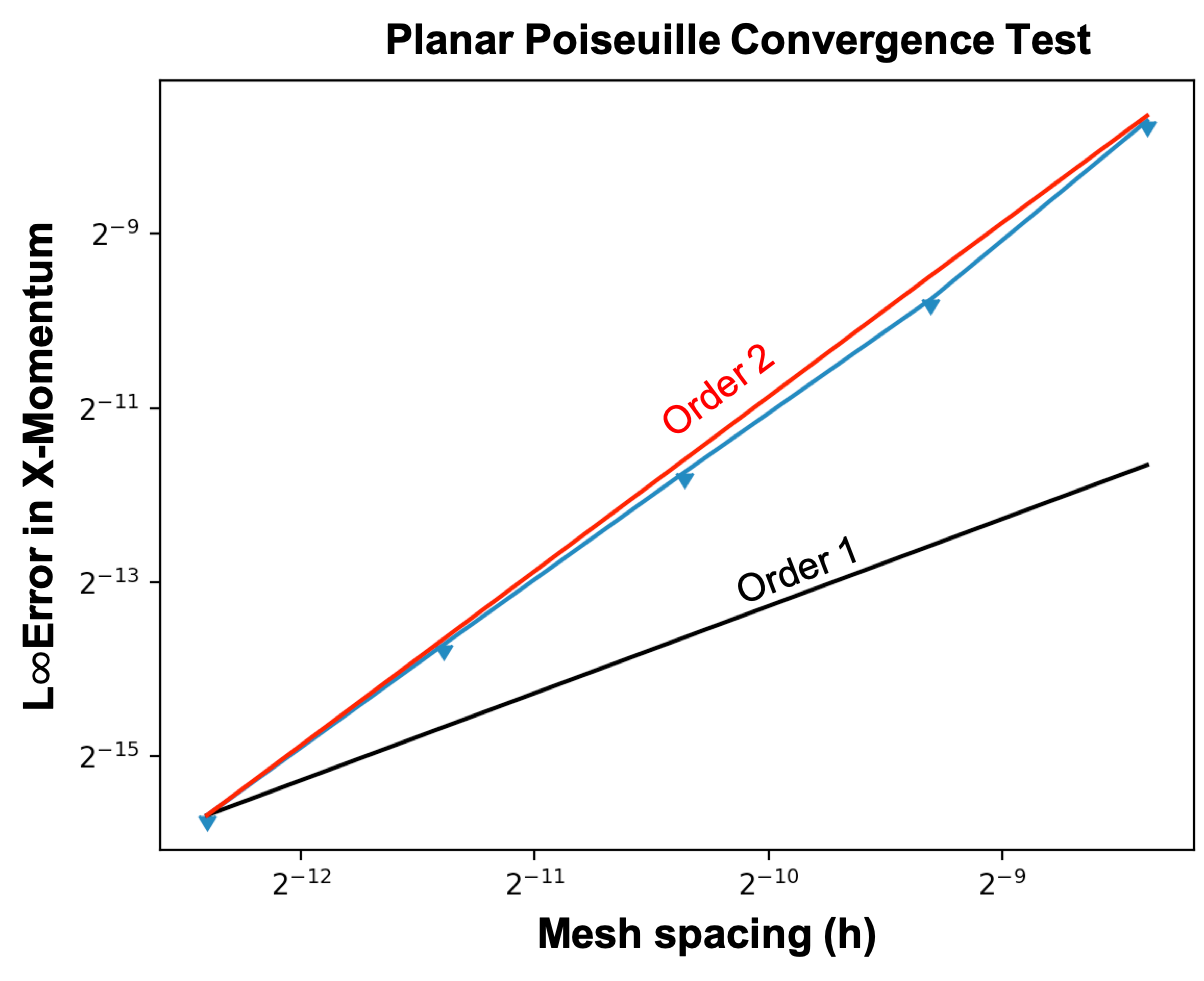
\includegraphics[width=.3\textwidth]{Figures/mtc/PoiseuilleConvergence2.png}
%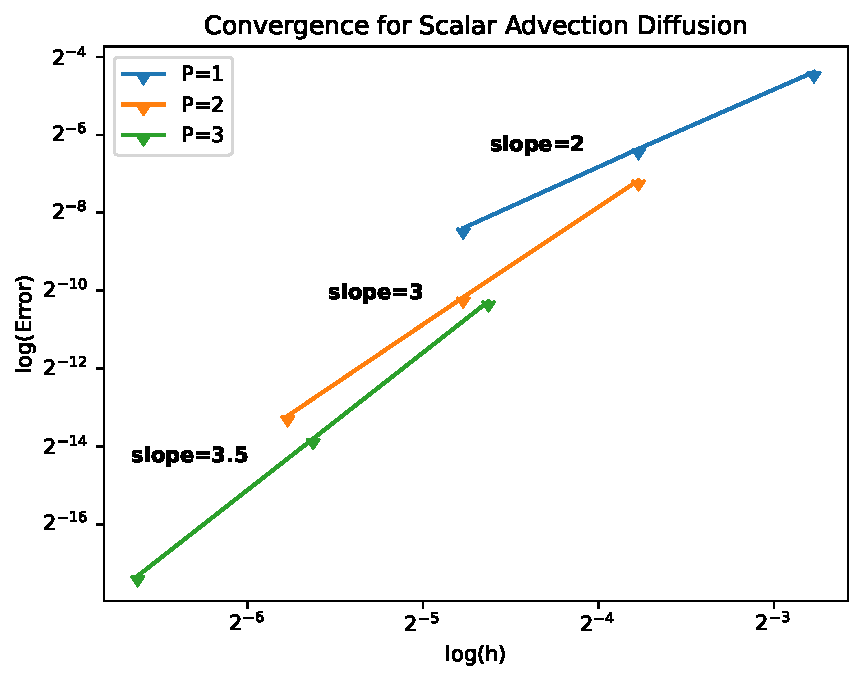
\includegraphics[width=.3\textwidth]{Figures/mtc/scalar_advdiff_convergence.pdf}
%\end{multicols}
%\end{frame}

